\documentclass[tikz]{standalone}
\usepackage{pgfplots}
\pgfplotsset{compat=1.15}
\usepackage{mathrsfs}
\usetikzlibrary{arrows,calc}
\usepackage{tkz-euclide}

\pagestyle{empty}

\definecolor{AngleClr}{rgb}{0,0.39215686274509803,0}
\definecolor{ShapeClr}{rgb}{0.6,0.2,0}

\begin{document}

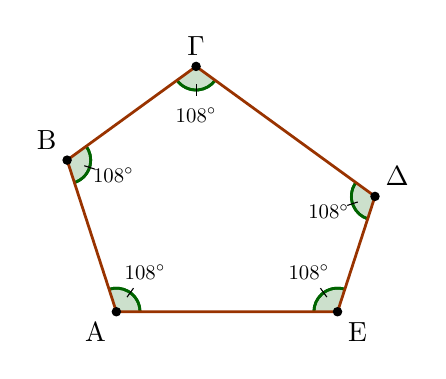
\begin{tikzpicture}[scale=.75]
\tkzSetUpLine[line width=1pt,color=black]
\tkzSetUpPoint[fill=black]

\tkzDefPoints{0/0/P0,2.7/0/P1,4.2/1.4/T}

\tkzDefRegPolygon[side,sides=5](P0,P1)

\tkzDefLine[parallel=through T](P2,P3) \tkzGetPoint{x}
\tkzInterLL(P1,P2)(T,x) \tkzGetPoint{Q2}
\tkzInterLL(P4,P3)(T,x) \tkzGetPoint{Q3}

\tkzFillPolygon[fill=white](P1,Q2,Q3,P4,P5)

\tkzFillAngles[fill=AngleClr,size=.4,fill opacity=0.2](Q3,Q2,P1 P4,Q3,Q2 P5,P4,Q3 P1,P5,P4 Q2,P1,P5)
\tkzMarkAngles[line width=1pt,size=.4,color=AngleClr](Q3,Q2,P1 P4,Q3,Q2 P5,P4,Q3 P1,P5,P4 Q2,P1,P5)
\tkzMarkAngles[mark=|,mksize=2,line width=1pt,size=.4,color=AngleClr](Q3,Q2,P1 P4,Q3,Q2 P5,P4,Q3 P1,P5,P4 Q2,P1,P5)

\tkzDrawPolygon[color=ShapeClr](P1,Q2,Q3,P4,P5)
\tkzDrawPoints[size=3](P1,Q2,Q3,P4,P5)
\tkzLabelPoint[below left](P1){$\rm A$}
\tkzLabelPoint[below right](Q2){$\rm E$}
\tkzLabelPoint[above right](Q3){$\rm \Delta$}
\tkzLabelPoint[above](P4){$\rm \Gamma$}
\tkzLabelPoint[above left](P5){$\rm B$}

\tkzLabelAngles[scale=0.75,pos=1.1](Q3,Q2,P1 P4,Q3,Q2 P5,P4,Q3 P1,P5,P4 Q2,P1,P5){$108^\circ$}

\end{tikzpicture}

\end{document}
